\documentclass{article}
\usepackage[a4paper, portrait, margin=1in]{geometry}
\usepackage{tabularx}
\usepackage{graphicx}
\usepackage{amsmath}
\usepackage{amsfonts}
\usepackage{algorithm}
\usepackage[noend]{algpseudocode}


\title{AIW \& Information Retrieval (UE18CS322)\\Unit 2}
\author{Aronya Baksy}
\date{February 2021}

\begin{document}
\maketitle
\section{Hardware Basics and BSBI}
\subsection{Hardware Basics}
\begin{itemize}
    \item The memory hierarchy of a system comprises of the registers, cache, RAM, ROM (magnetic drives, tape drives or SSDs) and peripheral storage (USB flash drives etc). 
    
    \item Registers are the fastest but also the most expensive per byte of memory. Hence registers are also the smallest in capacity.
    
    \item Registers are a subset of the cache, cache is a subset of the RAM and so on. 
    
    \item For a magnetic disk, the total memory access time comprises of seek time (time needed to move the disk head to the right cylinder), the transfer time (time needed to transfer bytes from disk to I/O controller) and the rotational latency (time needed for the right sector to fall under the disk head to be read). 
    
    \item Contiguous memory access is faster than accessing non-contiguous chunks of data. 
    
    \item The DMA controller controls the system bus that transfers data, hence the processor is free to process data during this operation. 
    
    \item An efficient set of compression and decompression algorithms can make the time needed to read compressed data much less than the time for uncompressed data. 
\end{itemize}

\subsection{Blocked Sort Based Indexing (BSBI)}
\begin{itemize}
    \item Sorting is a key step of inverted index construction (see Unit 1). Hence efficient sorting algorithm that takes memory structure into consideration is useful.
    
    \item An \textit{external sort algorithm} (one that uses data stored on secondary storage) is needed as large corpora will simply not work with internal sorting algorithms (that load all data into the main memory) 
    
    \item Terms are represented as integer term IDs (instead of strings). This puts an upper bound on the memory needed to store the terms in the inverted index. 
    
    \item The construction of the term - term ID mapping is either done during the inverted index construction (single pass approach) or done separately before the actual index construction (2-pass approach)
    
    \item The steps involved in BSBI are:
    \begin{enumerate}
        \item The algorithm parses documents into termID–docID pairs and accumulates the pairs inmemory until a block of a fixed size is full ($ParseNextBlock()$)
        
        \item The $BSBI\_Invert(block)$ function then sorts the termID–docID pairs and collects all termID–docID pairs with the same termID into a postings list where a posting is simply a docID.
        
        \item In the final step, the algorithm simultaneously merges the blocks into one large merged index
    \end{enumerate}
    
    \item Time complexity of BSBI is $\Theta(T log T)$ where $T$ is number of terms. 
    
    \item Merging process ($MergeBlocks()$) is outlined as follows:
    \begin{enumerate}
        \item Open each block file and maintain one read buffer for each
        
        \item Open the output file and maintain a single write buffer for it
        
        \item For each iteration:
        \begin{enumerate}
            \item Read from all read buffers simultaneously
            
            \item Select the lowest term ID that is not yet processed
            
            \item Read and merge all posting lists for this term ID
            
            \item Write this merged output using the write buffer
            
            \item Refill all read buffers when needed
        \end{enumerate}
    \end{enumerate}
    
    \item This merge minimizes number of disk seeks as it moves linearly through each block. 
    
    \item The limitations of BSBI are:
    \begin{itemize}
        \item It assumes that document corpus fits on disk
        
        \item It assumes that corpus is static
        
        \item The term-term ID mapping has to be carried in memory throughout the execution
    \end{itemize}
\end{itemize}

\begin{algorithm}[!t]
\caption{Blocked Sort-based Indexing Algorithm}
\begin{algorithmic}
    \Procedure{BSBI()}{}
    \State $n \leftarrow 0$
    \While{all docs not processed}
        \State $n \leftarrow n+1$
        \State $block \leftarrow ParseNextBlock()$
        \State $BSBI\_Invert(block)$
        \State $WriteToDisk(block, f_n)$
    \EndWhile
    \State $MergeBlocks(f_1, f_2, ..., f_n; f_{merged})$
    \EndProcedure
\end{algorithmic}
\end{algorithm}

\subsection{Single Pass In-Memory Indexing (SPIMI)}
\begin{itemize}
    \item BSBI scales well, but has disadvantages seen above. Also it involves the expensive step of sorting blocks and storing them, and storing the term-term ID mapping
    
    \item SPIMI uses the terms directly. The algorithm takes in a stream of $\langle$ term ID, doc ID $\rangle$ pairs that are generated from the document corpus. 
    
    \item The SPIMI algorithm comprises of the following steps:
    \begin{enumerate}
    
        \item Till main memory is exhausted work with the current block 
        \begin{enumerate}
            \item Sequentially access the documents. Let docID be the ID of the currently accessed document
                \begin{enumerate}
                    \item If the term is new, create a new entry for that term in the block dictionary
                    
                    \item Else identify the list for the term in the dictionary
                    
                    \item If the list is full double it's size
                \end{enumerate}
        \item Add doc ID to the posting list for the term.
        \end{enumerate}
        
        \item Sort on terms for lexicographical ordering
        
        \item Write index block into disk and start a new block and its corresponding fresh dictionary. 
    \end{enumerate}
    
    \item Posting lists here are dynamically growing, as against in BSBI where the posting list is constructed only once for all the term ID -doc ID pairs in a single block.
    
    \item Sorting of each block is done in order to facilitate the merging step
    
    \item Both the postings and the dictionary terms can be stored compactly on disk using compression.
    
    \item Compression increases the efficiency of the algorithm further because larger blocks can be processed, and because the individual blocks require less space on disk. 
    
    \item Same limitations as BSBI exist here too
    
\end{itemize}
\begin{algorithm}[!t]
\caption{Single Pass In-Memory Indexing}
\begin{algorithmic}
    \Procedure{SPIMI}{tokenStream}
    \State $outFile = New\_File()$
    \State $dict = New\_HashTable()$
    \While{memory is available}
        \State $token \leftarrow getNextToken(tokenStream)$
        \If{term(token) $\notin$ dict}
            \State PostingList = $addToDict(dict, term(token))$
        \Else
            \State PostingList = $getPostingList(dict, term(token))$
        \EndIf
        \If{full(PostingList)}
            \State PostingList = $doublePostingList(dict, term(token))$
        \EndIf
        \State AddToPostingList(PostingList, docID(token))
    \EndWhile
    \State sortedTerms $\leftarrow$ SortTerms(dict)
    \State WriteBlockToDisk(sortedTerms, dict, outFile)
    
    \Return outFile
    \EndProcedure
\end{algorithmic}
\end{algorithm}

\section{Distributed and Dynamic Indexing}

\subsection{Distributed Indexing}

\subsubsection{Map-Reduce and HDFS}
\begin{itemize}
    \item HDFS is a fault-tolerant distributed file system that offers high throughput access to data while being deployed on commodity hardware. 
    
    \item The key ideas behind HDFS are:
    \begin{itemize}
    
        \item Data \textbf{replicated across} multiple nodes for better fault tolerance
        
        \item \textbf{Move computation to the data} to address data locality and minimize network latency due to data transfer (traditional approaches would move the data towards the computation)
        
        \item Simple programming model that ensures minimal amount of data movement over the network
    \end{itemize}
    
    \item MapReduce is a programming framework that enables large computations over a distributed cluster. The generic framework is summarized as follows:
\end{itemize}
\begin{figure}[!h]
    \centering
    \begin{tabular}{|c|c|c|}
        \hline
        \textbf{Phase} & \textbf{Input} & \textbf{Output} \\
        \hline
        Map  &  $\langle k_1, v_1 \rangle,\langle k_2, v_2 \rangle, \langle k_3, v_3\rangle, ..., \langle k_n, v_n \rangle$ & $\langle \langle k_1, f(v_1) \rangle, \langle k_2, f(v_2) \rangle, ..., \langle k_n, f(v_n) \rangle \rangle $  \\
        \hline
        Shuffle & $\langle \langle k_1, f(v_1) \rangle, \langle k_2, f(v_2) \rangle, ..., \langle k_n, f(v_n) \rangle \rangle$ & $\langle k_1, \langle v_a, v_b, v_c\rangle, \langle k_2, \langle v_p, v_q, v_r, .. \rangle, ...  \rangle $ \\
        \hline
        Reduce & $\langle k_1, \langle v_a, v_b, v_c\rangle, \langle k_2, \langle v_p, v_q, v_r, .. \rangle,  ...  \rangle $ & $\langle k_1, v_{out1} \rangle, \langle k_2, v_{out2} \rangle, .. $ \\
        \hline
    \end{tabular}
\end{figure}
\begin{itemize}
        \item The \textbf{map} phase applies the map function on each value of the key-value pairs and outputs them.
    
        \item The \textbf{shuffle} phase takes input from map phase, and combines all the values under a single key into a list of values under that key.
        
        \item The \textbf{reduce} phase reduces the key, list of values pairs into key, value pairs.   
        
        \item The optional \textbf{partitioner} phase takes place after map and before reduce. The data is partitioned according to the defined partition funciton, and number of partitions is same as number of reducers. 
        
        \item The optional \textbf{combiner} phase pre-aggregates all the values of the same key within the mapper itself (rather than at the shuffle phase which has to take input from \textit{all the mappers}).
        
        \item The partitioner and combiner are optimizations that increase performance and reduce the data transfer over network. 
\end{itemize}

\subsubsection{Index construction using Map-Reduce}
\begin{itemize}
    \item The document collection is split into blocks called \textit{splits}. Splits are assigned to worker nodes by a master node. 
    
    \item The master node is also capable of restarting a job on a different node if a particular split is not behaving properly (too slow or just failed). 
    
    \item The \textbf{parser} (running on the mapper nodes) takes the documents and turns them into a stream of $\langle term, docID \rangle$ pairs. The parser writes them into the segment files (partitions)
    
    \item The segment files are made based on the first letter of the term and number of partitions $j$ (eg: if $j=3$ then one possible partition is a-f, g-p and q-z). 
    
    \item The \textbf{inverter} (running on the reducer node) collects all the postings for a single term, aggregates them into a list and returns the posting list as output for the term. 
    
    \item Each segment file requires only a sequential read as all data relevant to an inverter are only in written to a single segment file by the parser. This minimizes network traffic during indexing
    
    \item If term IDs are to be used instead of terms themselves, then the term-term ID mapping can be precomputed and stored on all the mapper nodes. 
    
    \item The current result is a term-partitioned index (wherein each reducer only handles a subset of the terms) as against a document-partitioned index (each reducer handles a subset of documents) which is preferred for many search engines. This involves a transformation step to be discussed later.  
\end{itemize}

\begin{figure}[!h]
    \centering
    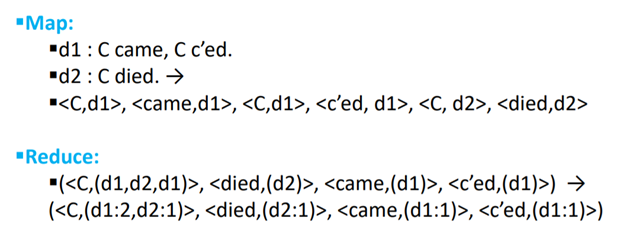
\includegraphics[scale=0.7]{img1.png}
    \caption{Map Reduce Index Construction}
    \label{fig:my_label}
\end{figure}

\subsection{Dynamic Indexing}
\begin{itemize}
    \item Indexing method for dynamic corpora (changing with time). 
    
    \item The simplest approach to dynamic indexing is as follows:
    \begin{enumerate}
        \item Maintain a single main index on disk
        
        \item Each time a document is added add it to an auxiliary index maintained in main memory. 
        
        \item Searching is carried out across both indices and the results are merged. 
        
        \item Periodically, the main and auxiliary indices have to be merged when the auxiliary index becomes too large for the main memory.
        
        \item A bit vector is maintained for all documents. When a document is deleted, its bit is flipped. The set of documents returned by a query is filtered according to this bit vector. 
        
    \end{enumerate}
    
    \item This strategy works well but has a few drawbacks:
    \begin{itemize}
        \item Frequent merging operations can be costly depending on how the main index is stored on the file system:
        \begin{itemize}
            \item If each posting list in the main index has its own file then merging is not very costly. 
            
            \item But each posting list in separate file means there are as many files as terms in the corpus. File system will not be able to handle so many open files.
            
            \item The alternative is to merge efficiently, and maintain large index files. (in this discussion it is assumed that the index is a single large file)
        \end{itemize}
    \end{itemize}
    
    \item This approach has complexity $\Theta (T^2/n)$ where $n$ is the size of the auxiliary index and $T$ is the number of postings. 
\end{itemize}

\subsubsection{Logarithmic Merging}
\begin{itemize}
    \item Maintain indices $I_0, I_1, I_2, .., I_n$ on disk where the size of index $I_i$ is $2^i \times n$ postings. 
    
    \item Upto $n$ postings are accumulated in the in-memory index called $Z_0$. When $Z_0$ becomes full, the $n$ postings in $Z_0$ are transferred to index $I_0$ on disk. 
    
    \item The next time that $Z_0$ becomes full, it is merged with $I_0$ to create $Z_1$. The size of $Z_1$ is $2^1\times n$.
    
    \item If there is no index $I_1$ on disk then $Z_1$ is stored to disk as $I_1$. But if $I_1$ exists on disk then $I_1$ and $Z_1$ are merged to create $Z_2$, and so on. 
    
    \item A query is serviced by checking $Z_0$ in memory as well as the indices $I_i$ on disk. The results are merged from all these $log(T/n)$ indices. 
    
    \item Overall index construction time is $\Theta(T log(T/n))$ because each posting is processed only once on each of the $log(T/n)$ levels.
\end{itemize}
\subsubsection{Dynamic Indexing: Real world applications}
\begin{itemize}
    \item Having multiple indexes complicates the maintenance of collection-wide statistics
    \begin{itemize}
        \item Affects spelling correction (querying multiple indexes + invalidation bit vector makes things more complicated)
        
        \item Dynamic indexing is implemented at large search engines with frequent small increments.
        
        \item Occasional complete rebuild of the index becomes harder with increasing size (e.g. Google would take several decades to rebuild its document index)
        
        \item During the complete rebuild, query processing is switched to the new index and the old index is deleted
    \end{itemize}
\end{itemize}

\section{Index Compression}
\begin{itemize}
    \item Compression saves disk space, increases speed (by keeping more information in memory) and saves on disk seeks needed to read large amt of uncompressed data. 
    
    \item Dictionary compression - keep in main memory, Index compression- reduce disk space and disk read latency
    
    \item Compression makes sense only if decompression algorithms are efficient.
    
    \item Lossy compression involves discarding some information. Techniques such as stop-word removal, stemming, downcasing, eliminating numbers are examples of lossy compression
    
    \item Lossless compression involves information being preserved even after the compressed data is decompressed. 
\end{itemize}

\subsection{Heap's Law and Zipf's Law}
\subsubsection{Heap's Law}
\begin{itemize}

    \item Heaps’ law is that the simplest possible relationship between collection size and vocabulary size is linear in log–log space
    
    \item Heap's Law models the number of unique terms $M$ as a function of the number of tokens in the collection $T$
    \begin{equation}
        M = k T^b
    \end{equation}
    where $30 \le k \le 100$ and $b \approx 0.5$
    
    \item In the log-log space, the Heap's law equation transforms to
    \begin{equation}
        log(M) = k + b\text{ }log(T)
    \end{equation}
    which is linear. 
    
    \item Heap's Law suggests that 
    \begin{enumerate}
    \item The dictionary size continues to increase with more documents in the collection, rather than a maximum vocabulary size being reached

    \item The dictionary size is large for large collections.
    \end{enumerate}
\end{itemize}

\subsubsection{Zipf's Law}
\begin{itemize}
    \item Zipf's law models the frequency distribution of terms in a document corpus. 
    
    \item Let $cf_i$ be the collection frequency of the $i^{th}$ most common term in the collection. Then Zipf's Law states that:
    \begin{equation}
        cf_i \propto \frac{1}{i}
    \end{equation}
    
    \item e.g. if the most frequent term has CF of $k$, then second most frequent will have CF $\frac{k}{2}$, third most frequent has $\frac{k}{3}$ and so on. 
    
    \item Zipf's Law is also a power law as it can be written as
    \begin{align}
                cf_i &= \frac{c}{i} \\
                log(cf_i) &= log(c) -\text{ }log(i)
    \end{align}
    
    \item Key insight from Zipf's law: Few frequent terms, many rare terms

\end{itemize}
    
\subsection{Dictionary Compression}
\subsubsection{Level 1}
\begin{itemize}
    \item Example corpus here is Reuters RCV1 with 400k terms. 
    \item Assume dictionary implemented as an array of fixed-width entries (20 bytes for term, 4 bytes for document frequency, and 4 bytes for ptr to posting list). Then for RCV1, the size is 11.2 MB
    
    \item Giving 20 bytes for word wastes space for majority of words and doesn't handle words larger than 20 chars long. 
    
    \item Average size of dictionary words is 8 chars. 
    
    \item Solution: Store all terms as one long string, sorted in lexical order. The pointer to the next term is also used to demarcate the end of the current term.
    
    \item Pointer has to distinguish up to 400k $\times$ 8 = 3.2 million positions. Hence needs to be 22 bytes $\rightarrow$ 3 bits long. 
    
    \item Now each entry is of size (4 for doc freq, 4 for posting ptr, 3 for term ptr, 8 for term) = 19 bytes, which leads to index size of 7.6 MB
\end{itemize}

\subsubsection{Level 2: Blocked Compression}
\begin{itemize}
    \item Divide string into blocks of size $k$ terms. Store only the pointer to the beginning of the block. In addition, at the beginning of each term in the string, store the length of the term in a single byte
    
    \item This saves $(k-1)\times 3$ bytes for term pointers, but adds $k$ bytes for the term lengths. (saving for each block)
    
    \item Assume $k=4$. Then saving per block is 5 bytes. Then saving overall is $\frac{400k \times 5}{4}$ which is 500kB. Hence new index size is 7.6-0.5 = 7.1 MB
    
    \item Disadvantage is that lookup speed decreases for large value of $k$ (even though large $k$ leads to more compression)
\end{itemize}

\subsubsection{Level 3: Front Coding}
\begin{itemize}
    \item Since the terms are sorted lexicographically, there are sequences of consecutive terms in the string that share the same prefix. 
    
    \item Once an unique prefix is identified, the end is denoted as *. In subsequent entries having that prefix it is denoted with $\Diamond$
    
    \item Experiments show that RCV1 dictionary size drops to 5.9 MB due to this
    
    \item e.g.: 8automat*a1$\Diamond$e2$\Diamond$ic3$\Diamond$ion
    
    \item Above denotes "automata, automate, automatic, automation"
\end{itemize}

\subsection{Posting List Compression}
\subsubsection{Level 1: Run Length Compression}
\begin{itemize}
    \item Instead of storing the posting list as a list of Doc IDs, store only the first doc ID and the rest of them as "gaps" between 2 doc IDs. (e.g. If the original list is 33, 47, 154, 159, 202 then the gap version is 33, 13, 107, 5, 43)
    
    \item Issue is that for rare words, gaps are large and need large space to store (almost as large as doc IDs themselves) but for frequent words this leads to lots of space saved. 
    
    \item A variable encoding method is used that needs fewer bits for short gaps.
\end{itemize}

\subsubsection{Variable Byte Codes}
\begin{itemize}
    \item The first bit (from the left) of each byte indicates whether that byte is the last byte of the current stream or not
    
    \item To convert any number from base 10 to its VB encoding, split into 7 bit substrings (from the rightmost string of 7 bits and then so on). Now at the head of each 7 bit string put 1 if it is the last byte or 0 if it is not
    
    \item This results in a sequence of 8-bit (byte) strings. 
    
    \item e.g. 829 in base 10 is represented as 11 0011 1101. 
    \begin{itemize}
        \item Split into 7 bit strings from the right (pad 0s where needed) gives 0000110 0111101
        
        \item Put 0 if byte is not last byte or 1 if it is last byte. This gives \textbf{0}0000110 \textbf{1}0111101. This is the VB encoded form of the number 829. 
    \end{itemize}
\end{itemize}

\subsubsection{Bit-Level Code (Gamma Code)}
\begin{itemize}
    \item An \textbf{unary} code is a bit-level code. (Unary code for $n$ is $n$ ones followed by a 0. e.g. unary code for 5 is 111110)
    
    \item The $\gamma$ code is a 2-tuple consisting of a length and an offset. For a value $G$, 
    \begin{enumerate}
        \item Offset is $G$ in binary with the leading bit removed. e.g. length of 13 is 1101 without the leading bit so 101
        
        \item Length is the length of the offset string, represented in Unary code. For 13, offset is 101 so length is 3, in unary that is 1110
        
        \item Hence the $\gamma$ code for 13 is (length, offset) which is (1110, 101)
    \end{enumerate}
    
    \item NOTE: 0 has no $\gamma$ code, the $\gamma$ code for 1 is 0. 
    
    \item The $\gamma$ code encodes a value $G$ in $2 \lfloor log_2(G) \rfloor +1 $ bits. 
    
    \item Just like the VB code, the $\gamma$ code is also uniquely prefix decodable. Read from L to R, as soon as you encounter a 0, you have reached the end of the length field. 
    
    \item $\gamma$ code can be used for any distribution (rare or common) and is independent of corpus size or any other parameters
\end{itemize}

\subsubsection{Implementation Notes}
\begin{itemize}
    \item Computer systems have word boundaries as powers of 2 bits. As $\gamma$ is a variable-bit length encoding scheme, it is impractical to use (operations that straddle a word bdy are slower)
    
    \item In this scenario VB code is more suitable as it is at the byte level, with only very small penalty in terms of space compared to $\gamma$ code. 
\end{itemize}

\section{Term Frequency, Weighting and Scoring}
\begin{itemize}
    \item Boolean queries tend to either come up with too many irrelevant results, or too few good ones. It is hard to craft a good Boolean query in this case. 
    
    \item In \textbf{ranked retrieval}, the system returns an ordering over the top documents that were retrieved for a query. A score (say in the range $[0, 1]$) is assigned to each document as a measure of its relevance to the query.
    
    \item Jaccard Similarity is useful as a scoring system. The drawbacks however are:
    \begin{itemize}
        \item Biased against longer sentences
        
        \item Doesn't consider term frequency information (rare terms contain more info than frequent terms)
    \end{itemize}
    
    \item The Bag-of-Words model treats each document as a vector of term counts. But it does not encode any position information
\end{itemize}
\subsection{TF-IDF Model}
\begin{itemize}
    \item \textbf{Term Frequency} $tf(t, d)$ is the number of times a term $t$ appears in a specific document $d$. 
    
    \item The weighted TF is given as 
    \begin{equation}
        w_{t, d} = \begin{cases}
            1 + log_{10}(tf_{t,d})\text{ if }tf_{t,d} > 0 \\
            0 \text{ if }tf_{t,d} = 0 \\
        \end{cases}
    \end{equation}
    
    \item The Document Frequency $df_t$ of a term $t$ over a document corpus $D$ is the number of documents that have atleast one occurrence of term $t$. 
    
    \item The \textbf{inverse document frequency} is the quantity 
    \begin{equation}
        idf_t = log_{10}\left(\frac{N}{df_t}\right)
    \end{equation}
    where $N$ is the number of documents.
    
    \item Hence the tf-idf weight is the product of tf and idf weights. 
    \begin{equation}
        W_{t, d, D} = (1 + log_{10}(tf_{t,d})) \times log_{10}\left(\frac{N}{df_t}\right)
    \end{equation}
    
    \item For a query $q$, the tf.idf score for a given document $d$ is 
    \begin{equation}
        score = \sum_{t \in q \cap d} tf.idf(t, d)
    \end{equation}
\end{itemize}

\subsection{Similarity Measures for Vector .Space models}
\begin{itemize}
    \item Euclidean distance is a bad idea because:
    \begin{itemize}
        \item  Euclidean distance is large for vectors of different lengths but they contain similar information with different magnitude
        
        \item e.g. Append document d to itself to make $d'$. The euclidean distance between $d$ and $d'$ may be v large but they are v similar semantically (the \textbf{angle} between them is 0)
    \end{itemize}
    
    \item Angles between vectors are measured in terms of cosine because cosine decreases as angle increases. Large angle leads to less similarity and less cosine, hence makes sense
    
    \item The cosine similarity between 2 vectors is given as
    
    \begin{equation}
        sim(v_1, v_2) = \frac{v_1 . v_2}{||v_1|| \times ||v_2||}
    \end{equation}
     
    \item The two vectors are \textbf{length normalized} before the cosine similarity is computed. This is so that the effect of the lengths of the 2 vectors is nullified, but the intensity of the content still remains. 
\end{itemize}

\begin{figure}[!h]
    \centering
    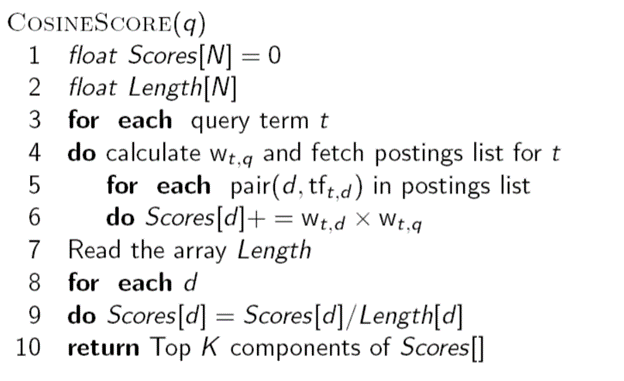
\includegraphics[scale=0.6]{p1.png}
    \caption{Algorithm for computing Cosine Similarity for a query $q$}
    \label{fig:my_label_1}
\end{figure}

\section{Efficient Scoring and Ranking}
\begin{itemize}
    \item TF-IDF matrix can be computed :
    \begin{itemize}
        \item One \textbf{Term at a Time} (TAAT). This involves summing over all the terms to get a document's score
        
        \item One \textbf{Document at a Time} (DAAT). This involves calculating tf-idf for one document at a time. 
    \end{itemize}
    
    \item A \textbf{safe ranking} is a method that guarantees that the $K$ documents returned are the absolute highest scoring documents. 
    
    \item A non safe ranking does not provide any such guarantees. However from the user perspective even an approximation is sufficient to provide results that are usable. 
    
    \item The generic approach is to select a set $A$ of size $K < |A| << N$. The set $A$ does not necessarily contain the top $K$, but has many docs from among the top $K$. Return the top $K$ docs in $A$
\end{itemize}
\subsection{Index Elimination}
\begin{itemize}
    \item One strategy is to \textit{eliminate terms with low IDF} from the query, as they don't contribute much to the final score but still have large number of associated documents 
    
    \item Another strategy is to only count \textit{documents containing many query terms}, for multi-term queries. Imposes a "soft conjunction" (implicit conjunction) on queries seen on web search engines
\end{itemize}

\subsection{Champion Lists}
\begin{itemize}
    \item For each dictionary term $t$, precompute the $r$ highest weighted documents in the posting list of $t$. This list is the champion (aka fancy) list for $t$. 
    
    \item It is possible that $r<K$ as the champion list is built during the index construction.
    
    \item  At query time, only compute scores for docs in the champion list of some query term, and pick the $K$ top-scoring docs from amongst these
\end{itemize}

\subsection{Static Quality Score}
\begin{itemize}
    \item Documents can be ranked across the dimensions of relevance (using cosine similarity) and authority (using some query independent parameter)
    
    \item Measures of authority include number of Wikipedia links, number of bit.ly etc. links, number of citations, normalized into a range between 0 and 1. 
    
    \item This authority measure for a document is denoted as a goodness score $g(d)$. The overall score for a term-document pair is $cosine(t,d) + g(d)$
    
    \item Ordering posting list for terms by $g(d)$ allows top $K$ documents to be retrieved earlier, thus allowing concurrent traversal for intersection as well as cosine similarity computation
    
    \item The idea of champion list is also combined with the goodness score. • Maintain for each term a champion list of the $r$ docs with highest $g(d) + tf-idf_{t,d}$
    
    \item Seek top-K results from only the docs in these ordered champion lists
\end{itemize}

\subsection{Impact-Ordered Postings}
\begin{itemize}
    \item Sort each postings list by tf-idf weight $wf_{t,d}$. 
    
    \item Follow the same algorithm but suitably modify for storing the partial scores for each doc as not all postings are in a common order
\end{itemize}
\subsubsection{Early Termination}
\begin{itemize}
    \item When traversing t’s postings, stop early after either
    \begin{itemize}
        \item a fixed number of r docs
        \item wft,d drops below some threshold
    \end{itemize}
    \item Take the union of the resulting sets of docs (one doc list from each query term)
    
    \item Compute only the scores for docs in this union
\end{itemize}

\subsubsection{idf Ordered Terms}
\begin{itemize}
    \item High idf terms are more likely to contribute to the highest ranking documents. Hence look at query terms ordered by their IDF. 
    
    \item As the document score is updated for each term, if the score remains almost constant then stop traversing the query terms. 
\end{itemize}

\subsection{High and Low List}
\begin{itemize}
    \item For each term, the high list is the champion list. 
    
    \item For each query term, traverse the docs in the high list first. If more than $K$ documents are retrieved then get the top $K$ and stop, else continue on to the low list
    
    \item This strategy can be used even for simple cosine scores, without global quality $g(d)$
\end{itemize}

\subsection{Cluster Pruning}
\begin{itemize}
    \item Pick $\sqrt{N}$ documents as cluster centres or leaders. Cluster the documents about these leaders. By this arrangement now each leader has $\sqrt{N}$ followers.
    
    \item Given query $Q$, find its nearest leader $L$, and seek K nearest docs from among $L$’s followers
    
    \item Leaders chosen at random are more likely to reflect the real data distribution. 
    
    \item Modifications: 
    \begin{itemize}
        \item Bring more “fuzziness” into the method, have each follower attached to $b_1=3$ (say) nearest leaders.
        
        \item From query, find $b_2=4$ (say) nearest leaders
        
        \item Since each follower can attach to $b_1$ leaders, we are now looking at a larger set of followers.
        
        \item Recursive leader-follower construction. 
    \end{itemize}
\end{itemize}

\subsection{Parameterized and Zoned Indices}
\begin{itemize}
    \item A document is more than a stream of tokens. It contains field each having its own syntax (Author, Year, Title, Language, Format), and these fields comprise the metadata of the document
    
    \item Field or parametric index: postings for each field value
    
    \item A zone is a region of the doc that can contain an arbitrary amount of text, e.g., Title, Abstract, References. Build inverted indexes on zones as well to permit querying
    
    \item This can be implemented as:
    \begin{enumerate}
        \item Having zone-specific tokens in the vocabulary (e..g "william.abstract" and "william.title" specify the term "william" occuring in the abstract and title of a dopcument)
        
        \item Single term but posting contains only the doc id but also the zone information
    \end{enumerate}
\end{itemize}

\subsection{Tiered Index}
\begin{itemize}
    \item Break postings up into a hierarchy of lists (from most to least important), ordered by measure like $g(d)$
    
    \item Inverted index thus broken up into tiers of decreasing importance

    \item At query time use top tier unless it fails to yield $K$ docs, if so drop to lower tiers
\end{itemize}

\subsection{Free Text Queries}
\begin{itemize}
    \item Combination of phrase queries, sub-phrase (2 words at a time and so on) and vector space queries. 
    
    \item The latter 2 are run only if the documents returned till that time are less than $K$
    
    \item Rank matching docs by vector space scoring
    
    \item Combination of multiple scoring algorithms (proximity, similiarity, static quality) done using expert-tuned approaches or using supervised machine learning approaches. 
\end{itemize}

\section{Components of an IR System}
\begin{itemize}
    \item Tokenization and normalization
    
    \item  Processed output of step 1 in cache for generating snippets used in retrieval results
    
    \item Multiple indexes are built (can be more than four. Inexact means optimized and k-gram index is useful for spellingcorrection ) in parallel
    
    \item Query parser submits query to the indexes

    \item Query parser also submits query after spelling correction
    
    \item Final score is aggregated using ML
\end{itemize}
\begin{figure}[!h]
    \centering
    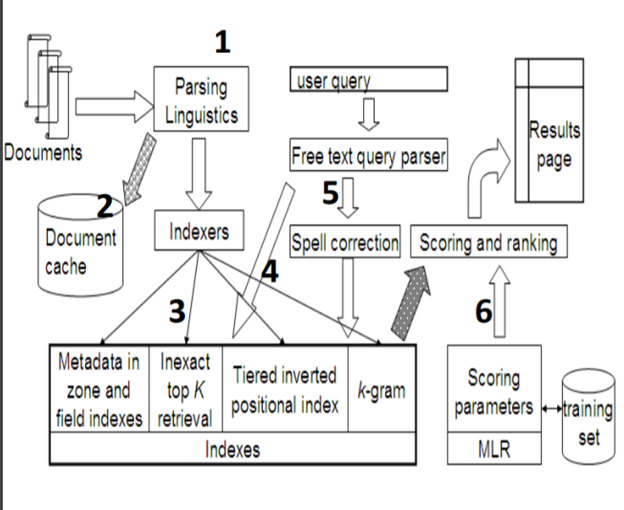
\includegraphics[scale=0.6]{p2.png}
    \caption{A complete IR System}
    \label{fig:my_label_2}
\end{figure}
\end{document}

